\documentclass[12pt,a4paper,utf8]{ctexart}
\usepackage{graphicx}
\usepackage{float}
\usepackage{amsmath}
\usepackage{amssymb}
\usepackage{subfig}
\usepackage{cite}
\usepackage[ntheorem]{empheq}
\usepackage{enumitem}
\usepackage{fullpage}
\usepackage{cleveref}
\usepackage{cellspace}
\usepackage{listings}
\usepackage{color}
\definecolor{gray}{rgb}{0.5,0.5,0.5}
\definecolor{dkgreen}{rgb}{.068,.578,.068}
\definecolor{dkpurple}{rgb}{.320,.064,.680}

% set Matlab styles
\lstset{
   language=Matlab,
   keywords={break,case,catch,continue,else,elseif,end,for,function,
      global,if,otherwise,persistent,return,switch,try,while},
   basicstyle=\ttfamily,
   keywordstyle=\color{blue}\bfseries,
   commentstyle=\color{dkgreen},
   stringstyle=\color{dkpurple},
   backgroundcolor=\color{white},
   tabsize=4,
   showspaces=false,
   showstringspaces=false
}

\begin{document}
\CJKfamily{zhkai}

\begin{center}
\textbf{作业三}\\
\textbf{姓名 ~何春望~ 学号 ~PB17000075~ 日期 ~2020.12.31}\\
\end{center}
\textit{}
\vspace{\baselineskip}

\begin{enumerate}
\item[第一题] 
\subitem(a)
对$i,j > 1$,
\begin{equation}
    \begin{aligned}
        a_{ij}^{(1)} &= a_{ij} - a_{1j} \cdot a_{i1}/a_{11}\\
        a_{ji}^{(1)} &= a_{ji} - a_{1i} \cdot a_{j1}/a_{11}\\
        &= a_{ij} - a_{1j} \cdot a_{i1}/a_{11}\\
        &= a_{ij}^{(1)}
    \end{aligned}
\end{equation}
故$\mathbf{A}^{(1)}$是对称的。

\subitem(b)
令$\mathbf{L} = \begin{bmatrix}
    1 \\
    \ell_{21} & 1 \\
    \ell_{31} & \ell_{32} & 1 \\
    \cdots & \cdots & \cdots & \ddots \\
    \ell_{n1} & \ell_{n2} & \cdots & \ell_{n n-1} & 1
\end{bmatrix}$,$\mathbf{D} = \begin{bmatrix}
    d_1 \\
    & d_2 \\
    && d_3 \\
    &&& \ddots \\
    &&&& d_n
\end{bmatrix}$,\\
则有$\mathbf{A}=\mathbf{L}\mathbf{U}=\mathbf{L}\mathbf{D}\mathbf{L}^\intercal$。
可通过以下伪代码解得所有未知量:

\text{for k = 1 to n: }

\text{\{ }

\text{~~~~$d_k = a_{kk} - \sum_{m=1}^{k-1} u_{km} \cdot \ell_{km}$ }

\text{~~~~for j = k+1 to n: }

\text{~~~~\{ }

\text{~~~~~~~~$\ell_{jk} = \left(a_{jk} - \sum_{m=1}^{k-1} \ell_{jm} \ell_{km} d_m\right)/d_k$ }

\text{~~~~\} }

\text{\} }

\subitem(c)
\textsc{Matlab}程序如下:
\begin{lstlisting}[frame=single]
clear, clc
A = [4, -2, 4, 2;
    -2, 10, -2, -7;
    4, -2, 8, 4;
    2, -7, 4, 7];
b = [8;2;16;6];
n=length(b);
L = zeros(n,n);

for j = 1:n
    for k = 1:j-1
        L(j,j) = L(j,j) + L(j,k)^2;
    end
    L(j,j) = sqrt(A(j,j) - L(j,j));
    for i = j+1:n
        for k = 1:j-1
            L(i,j) = L(i,j) + L(i,k)*L(j,k);
        end
        L(i,j)=(A(i,j)-L(i,j))/L(j,j);
    end
end

y=zeros(n,1);
y(1) = b(1) / L(1,1);
for i = 2:n
    for k = 1:i-1
        y(i) = y(i) + L(i,k)*y(k);
    end
    y(i) = (b(i)-y(i)) / L(i,i);
end

x=zeros(n,1);
x(n) = y(n) / L(n,n);
for i = n-1:-1:1
    for k = i+1:n
        x(i) = x(i) + L(k,i)*x(k);
    end
    x(i) = (y(i)-x(i)) / L(i,i);
end

x
\end{lstlisting}

程序输出$x=(1,2,1,2)'$。


\item[第二题]
\subitem(a)

$M^{-1}=\omega I$ \\
$x^{(k+1)}=(I-\omega A)x^{(k)} + \omega Ib$ \\
若要收敛,则需
$\rho(I-\omega A)=|1-\omega \lambda_n| < 1$ \\
即
$\omega \lambda_n - 1 < 1$ \\
故
$\omega < 2/\lambda_n$

\subitem(b)
$\omega$的最佳值需要使谱半径最小,而$\rho(G_\omega) = max(1-\omega \lambda_1, \omega\lambda_n-1)$

故令$1-\omega \lambda_1 = \omega\lambda_n-1$,解得$\omega_b=\frac{2}{\lambda_1+\lambda_n}$。\\
且$\rho(G_\omega)=\left\{\begin{array}{ll}
1-\omega\lambda_1 & \omega \leq \omega_b \\
\frac{\lambda_n-\lambda_1}{\lambda_n+\lambda_1} & \omega=\omega_b \\
\omega\lambda_n-1 & \omega\geq\omega_b
\end{array}\right.$

\subitem(c)
\textsc{Matlab}程序如下:
\begin{lstlisting}[frame=single]
clear, clc, clf
MS = 'MarkerSize'; ms = 10;
V = diag([1,2,3,4,5]);
U = orth(rand(5));
A = U*V*U';
b = rand(5,1);

lambda_n = max(eig(A));
lambda_1 = min(eig(A));
omega_b = 2 / (lambda_1+lambda_n);
delta_w = 1e-2;
epsilon = 1e-6;
for omega = delta_w:delta_w:2/lambda_n-delta_w
    M = eye(5) / omega;
    N = M - A;
    x = zeros(5,1);
    x_new = ones(5,1);
    while(max(abs(x_new - x)) > epsilon)
        x = x_new;
        x_new = M \ N * x + M \ b;
    end
    max_err = max(abs(x_new - A\b))

    if omega < omega_b
        rho_equa = 1 - omega*lambda_1;
    elseif omega > omega_b
        rho_equa = omega*lambda_n - 1;
    else
        rho_equa=(lambda_n-lambda_1)/(lambda_n+lambda_1);
    end
    rho_Gw = max(abs(eig(M\N)));
    
    plot(omega, rho_Gw, 'r.', MS, ms), hold on
    plot(omega, rho_equa, 'ko', MS, ms)
    xlabel('omega')
    ylabel('rho')
    legend('rho-Gw', 'rho-equation', 'location', 'sw')
    hold on
end
\end{lstlisting}

程序输出 max\_err = 4.6864e-07,谱半径随$\omega$变化:

\begin{figure}[H]
    \centering
    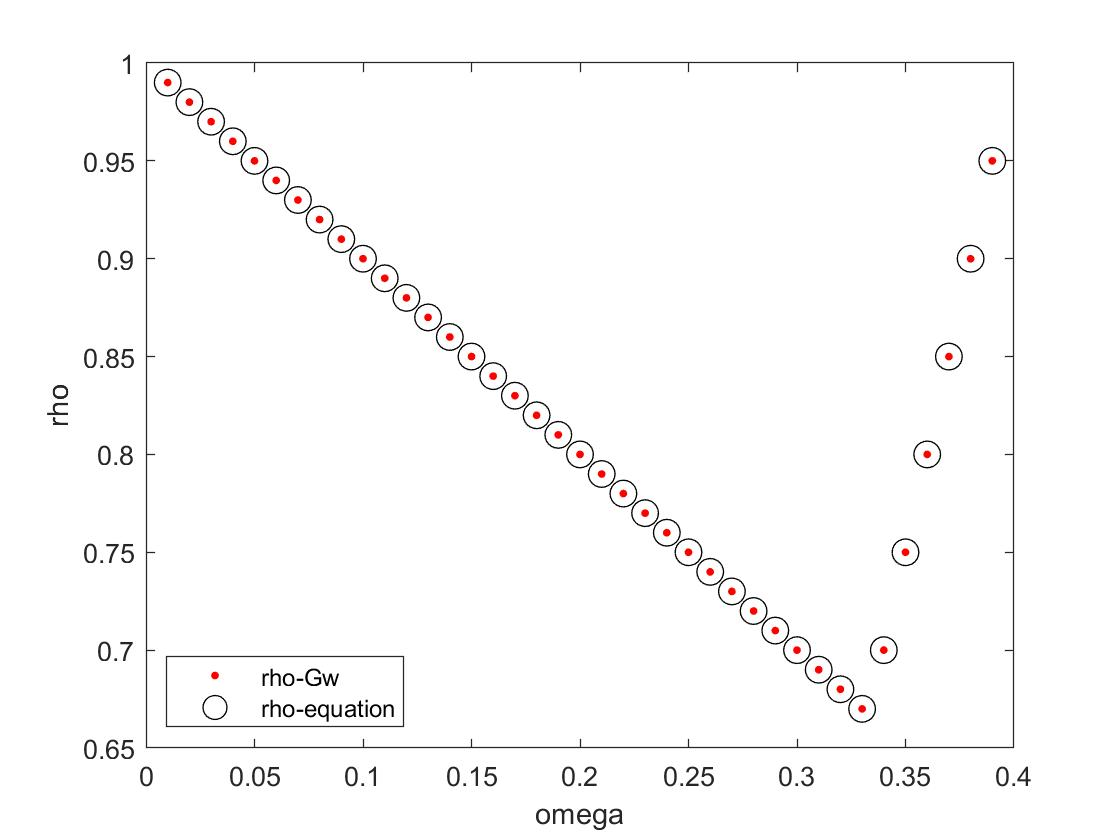
\includegraphics[width = .8\textwidth]{2c.jpg}
    \caption{谱半径随$\omega$变化}
\end{figure}


\item[第三题]
\subitem(a)
\begin{equation}
    \left\{\begin{array}{ll}
        c_1+c_2+c_3+c_4+c_5+c_6 &= \int_{-1}^1 1 \mathrm{d}x = 2\\
        c_1 x_1^2 + c_2 x_2^2 + c_3 x_3^2 + c_4 x_4^2 + c_5 x_5^2 + c_6 x_6^2 &= \int_{-1}^1 x^2 \mathrm{d}x = \frac{2}{3}\\
        c_1 x_1^4 + c_2 x_2^4 + c_3 x_3^4 + c_4 x_4^4 + c_5 x_5^4 + c_6 x_6^4 &= \int_{-1}^1 x^4 \mathrm{d}x = \frac{2}{5}\\
        c_1 x_1^6 + c_2 x_2^6 + c_3 x_3^6 + c_4 x_4^6 + c_5 x_5^6 + c_6 x_6^6 &= \int_{-1}^1 x^6 \mathrm{d}x = \frac{2}{7}\\
        c_1 x_1^8 + c_2 x_2^8 + c_3 x_3^8 + c_4 x_4^8 + c_5 x_5^8 + c_6 x_6^8 &= \int_{-1}^1 x^8 \mathrm{d}x = \frac{2}{9}\\
        c_1 x_1^{10} + c_2 x_2^{10} + c_3 x_3^{10} + c_4 x_4^{10} + c_5 x_5^{10} + c_6 x_6^{10} &= \int_{-1}^1 x^{10} \mathrm{d}x = \frac{2}{11}\\
        x_1 + x_6 = 0 \\
        x_2 + x_5 = 0 \\
        x_3 + x_4 = 0 \\
        c_1 = c_6 \\
        c_2 = c_5 \\
        c_3 = c_4
    \end{array}\right.
\end{equation}

\subitem(b)
利用对称性简化为
\begin{equation}
    \left\{\begin{array}{ll}
        c_1+c_2+c_3-1 &= 0\\
        c_1 x_1^2 + c_2 x_2^2 + c_3 x_3^2 - \frac{1}{3} &= 0\\
        c_1 x_1^4 + c_2 x_2^4 + c_3 x_3^4 - \frac{1}{5} &= 0\\
        c_1 x_1^6 + c_2 x_2^6 + c_3 x_3^6 - \frac{1}{7} &= 0\\
        c_1 x_1^8 + c_2 x_2^8 + c_3 x_3^8 - \frac{1}{9} &= 0\\
        c_1 x_1^{10} + c_2 x_2^{10} + c_3 x_3^{10} - \frac{1}{11} &= 0\\
    \end{array}\right.
\end{equation}

\begin{equation}
    J(x_1,x_2,x_3,c_1,c_2,c_3)=
    \begin{vmatrix}
        0 & 0 & 0 & 1 & 1 & 1\\
        2c_1 x_1 & 2c_2 x_2 & 2c_3 x_3 & x_1^2 & x_2^2 & x_3^2\\
        4c_1 x_1^3 & 4c_2 x_2^3 & 4c_3 x_3^3 & x_1^4 & x_2^4 & x_3^4\\
        6c_1 x_1^5 & 6c_2 x_2^5 & 6c_3 x_3^5 & x_1^6 & x_2^6 & x_3^6\\
        8c_1 x_1^7 & 8c_2 x_2^7 & 8c_3 x_3^7 & x_1^8 & x_2^8 & x_3^8\\
        10c_1 x_1^9 & 10c_2 x_2^9 & 10c_3 x_3^9 & x_1^{10} & x_2^{10} & x_3^{10}\\
    \end{vmatrix}
\end{equation}

\subitem(c)
\textsc{Matlab}程序如下:
\begin{lstlisting}[frame=single]
clear, clc
x = linspace(-1,1,6)';
c = ones(6,1);
w = [x(1:3); c(1:3)];

epsilon = 1e-6;
deltaw = ones(6,1);
while(max(abs(deltaw)) > epsilon)
    deltaw = jacob(w(1),w(2),w(3),w(4),w(5),w(6)) \...
                f(w(1),w(2),w(3),w(4),w(5),w(6));
    w = w + deltaw;
end
x = [w(1:3);-w(3:-1:1)]
c = [w(4:6); w(6:-1:4)]

function y = f1(x1,x2,x3,c1,c2,c3)
    y = c1+c2+c3-1;
end
function y = f2(x1,x2,x3,c1,c2,c3)
    y = c1*x1^2 + c2*x2^2 + c3*x3^2 - 1/3;
end
function y = f3(x1,x2,x3,c1,c2,c3)
    y = c1*x1^4 + c2*x2^4 + c3*x3^4 - 1/5;
end
function y = f4(x1,x2,x3,c1,c2,c3)
    y = c1*x1^6 + c2*x2^6 + c3*x3^6 - 1/7;
end
function y = f5(x1,x2,x3,c1,c2,c3)
    y = c1*x1^8 + c2*x2^8 + c3*x3^8 - 1/9;
end
function y = f6(x1,x2,x3,c1,c2,c3)
    y = c1*x1^10 + c2*x2^10 + c3*x3^10 - 1/11;
end

function y = jacob(x1,x2,x3,c1,c2,c3)
    y = [
        0,0,0,1,1,1;
        2*c1*x1, 2*c2*x2, 2*c3*x3, x1^2, x2^2, x3^2;
        4*c1*x1^3, 4*c2*x2^3, 4*c3*x3^3, x1^4, x2^4, x3^4;
        6*c1*x1^5, 6*c2*x2^5, 6*c3*x3^5, x1^6, x2^6, x3^6;
        8*c1*x1^7, 8*c2*x2^7, 8*c3*x3^7, x1^8, x2^8, x3^8;
        10*c1*x1^9,10*c2*x2^9,10*c3*x3^9,x1^10,x2^10,x3^10;
    ];
end

function y = f(x1,x2,x3,c1,c2,c3)
    y = -[
        f1(x1,x2,x3,c1,c2,c3);
        f2(x1,x2,x3,c1,c2,c3);
        f3(x1,x2,x3,c1,c2,c3);
        f4(x1,x2,x3,c1,c2,c3);
        f5(x1,x2,x3,c1,c2,c3);
        f6(x1,x2,x3,c1,c2,c3);
    ];
end
\end{lstlisting}

程序输出\\
积分节点x = (-0.9325, -0.6612, -0.2386, 0.2386, 0.6612, 0.9325)',\\
积分权重c = (0.1713, 0.3608, 0.4679, 0.4679, 0.3608, 0.1713)'

\subitem(d)
\textsc{Matlab}程序如下:
\begin{lstlisting}[frame=single]
clear, clc,clf
MS = 'MarkerSize'; ms = 10;
F = @(x) x.^2.*cos(x);
% gauss.m
[x, w] = gauss(20);
I = w * F(x);

% cheb
epsilon = 1e-6;
for n = 1:20
    tmp = ceil(n/2);
    x = cos(linspace(pi,0,n))';
    c = ones(1,n);
    w = [x(1:tmp); c(1:tmp)'];
    
    deltaw = ones(2*tmp,1);
    while(max(abs(deltaw)) > epsilon)
        deltaw = jacob(n,w(1:tmp),w(tmp+1:end)') \...
                    f(n,w(1:tmp),w(tmp+1:end)');
        w = w + deltaw;
    end
    
    for i = 1:tmp
        x(i) = w(i);
        x(end-i+1) = -w(i);
        c(i) = w(tmp+i);
        c(end-i+1) = w(tmp+i);
    end
    semilogy(n, abs(c*F(x)-I), 'r.', MS, ms)
    xlabel('sampling point n')
    ylabel('Abs err')
    hold on
end

function y = f(n, x, c)
    y = zeros(n,1);
    for i = 1:n
        y(i) = c * (x.^(2*(i-1))) - 1/(2*i-1);
        if i == 1 && mod(n,2)
            y(i) = y(i) - c(end)/2;
        end
    end
    y = -y;
end

function y = jacob(n, x, c)
    tmp = ceil(n/2);
    y = zeros(n, 2*tmp);
    for i = 1:n
        for j = 1:tmp
            y(i,j) = 2*(i-1)*c(j)*x(j)^(2*(i-1)-1);
            y(i,j+tmp) = x(j)^(2*(i-1));
        end
    end
    if mod(n,2)
        y(:,end) = y(:,end)/2;
    end
end

function [x,w] = gauss(N)
    beta = .5./sqrt(1-(2*(1:N-1)).^(-2));
    T = diag(beta,1) + diag(beta,-1);
    [V,D] = eig(T);
    x = diag(D); [x,i] = sort(x);
    w = 2*V(1,i).^2;
end
\end{lstlisting}

\begin{figure}[H]
    \centering
    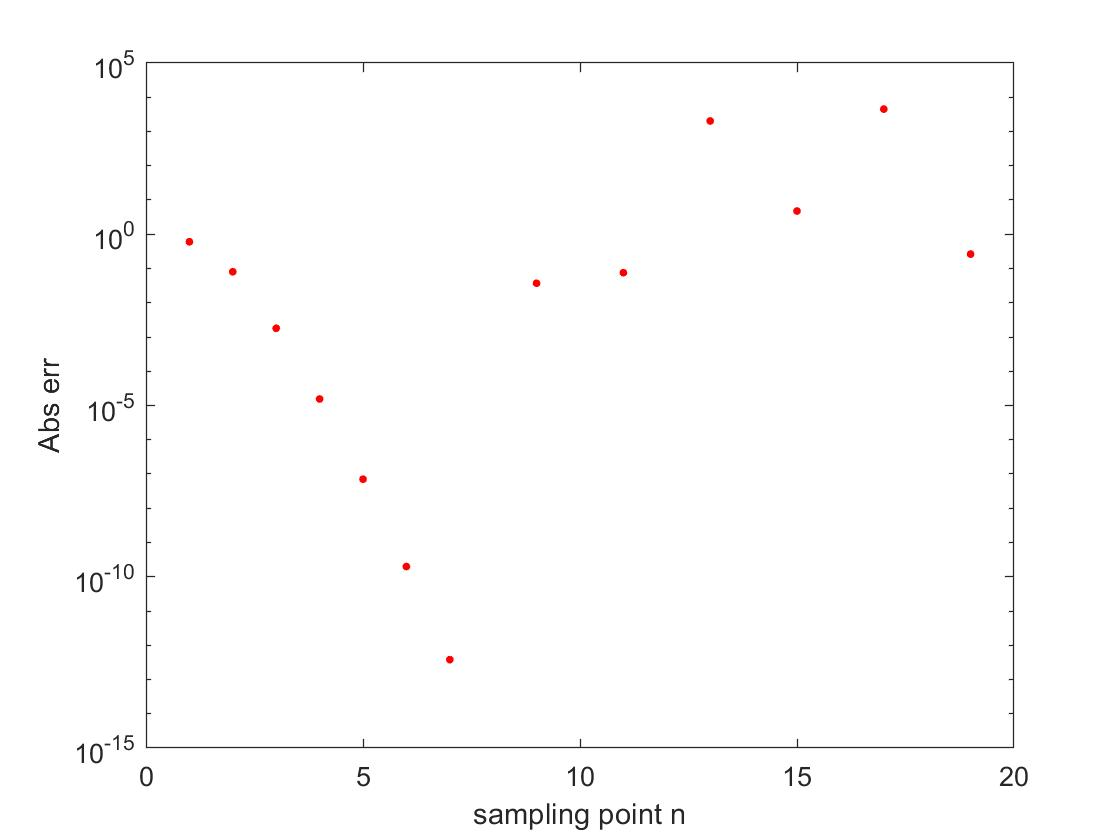
\includegraphics[width = .8\textwidth]{3d.jpg}
    \caption{积分误差随采样点数变化}
\end{figure}

由图可知最大采样点数为7。

\end{enumerate}

\end{document}
